\chapter{Resultados}   
\minitoc

\section{Propiedades \'opticas de algunas mol\'eculas $\pi$ conjugadas}

En la figura \ref{muchacha} se muestra una estructura de bajo peso molecular con un grupo de 15 sustituyentes distintos $R$ en dos de sus extremos; este conjunto de mol\'eculas fue estudiado en soluci\'on y suspensi\'on. La concentraci\'on de las soluciones y suspensiones acuosas fue del orden de $10^{-5} M$ y en la fabricaci\'on de las mismas se utiliz\'o Trit\'on X- 100 como surfactante, debido a que se observaron mejores resultados que utilizando CTAB (Suspensiones m\'as transparentes y estables).

No todas las mol\'eculas fueron solubles en THF, tampoco se pudieron fabricar suspensiones acuosas de nanopart\'iculas en todos los casos porque se formaban grandes aglomerados que se precipitaban y en algunos casos la emisi\'on lineal fue d\'ebil. En la figura \ref{abshgo} se muestran los espectros de absorci\'on lineal molar $\epsilon$ de las soluciones y suspensiones m\'as estables que presentaron mayor emisi\'on, en \'estos se puede observar el esparcimiento de las suspensiones. La absorci\'on disminuy\'o notoriamente en la mol\'ecula 7 en suspensi\'on comparada con la soluci\'on, mientras que para la mol\'ecula 3 el espectro de absorci\'on  de la suspensi\'on present\'o mayor intensidad de emisi\'on, un corrimiento hacia el rojo y ensanchamiento (debido a la torsi\'on y/o flexi\'on que sufre la mol\'ecula) en comparaci\'on con la soluci\'on.

\begin{figure}[h]
\centering
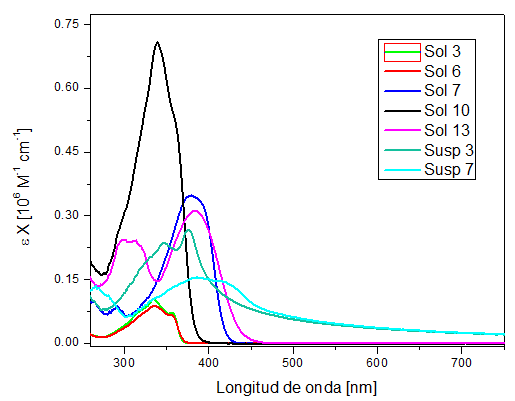
\includegraphics[width=0.9\textwidth]{resultados/sechgo/abstodas}
\caption{Espectros de absorci\'on molar de las mol\'eculas 3, 6, 7, 10, 13 y 15 (Notaci\'on de acuerdo a la fig. \ref{muchacha}). Las etiquetas \emph{Sol} y \emph{Susp} se refieren a las mol\'eculas en soluci\'on y suspensi\'on respectivamente.}\label{abshgo}
\end{figure}

En la figura \ref{emilinhgo} se muestran los espectros de emisi\'on lineal. El espectro de la soluci\'on 6 present\'o una intensidad mayor que la soluciones 10 y 13, sin embargo, se traslap\'o con la emisi\'on del diodo l\'aser de 370 $nm$ y como se utiliz\'o un filtro UV para no detectar la fuente de excitaci\'on, el espectro de la soluci\'on 6 no se pudo visualizar por completo. Lo mismo sucedi\'o para el espectro de la mol\'ecula 3 en soluci\'on, mientras que en suspensi\'on tuvo un corrimiento hacia el rojo por las interacciones que sufre la mol\'ecula al confinarse para formar las nanopart\'iculas. El espectro de la mol\'ecula 7 en suspensi\'on tambi\'en sufri\'o un corrimiento hacia el rojo comparado con el espectro en soluci\'on.

Como las mol\'eculas 3, 6, 7, 10 y 13 en soluci\'on presentaron la mayor intensidad de emisi\'on lineal, pudiendo disolverse f\'acilmente en THF y las mol\'eculas 3 y 7 formaron las suspensiones acuosas m\'as transparentes y estables (Ver Figura \ref{susphgo}), \'unicamente se midi\'o la eficiencia cu\'antica de fluorescencia para estas mol\'eculas; los resultados se muestran en la tabla \ref{tablahgo}.




\begin{figure}[H]
\centering
\begin{subfigure}{\textwidth}
\centering
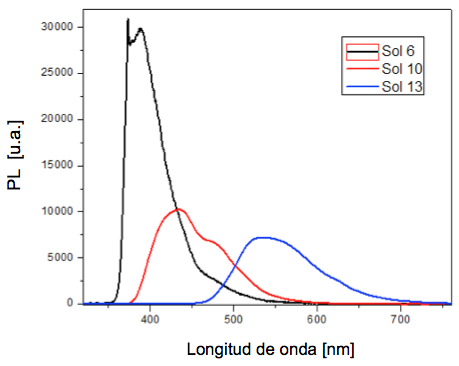
\includegraphics[width=0.65\textwidth]{resultados/sechgo/emlinsol}
\end{subfigure}
\begin{subfigure}{\textwidth}
\centering
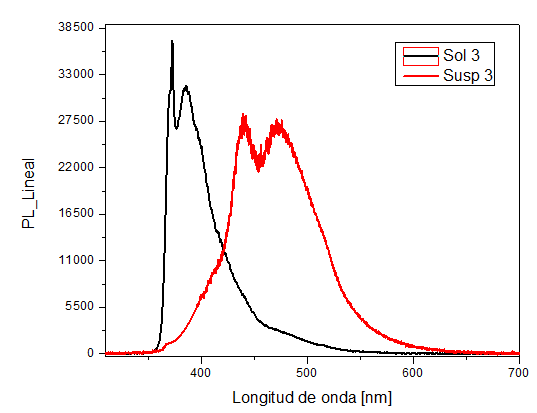
\includegraphics[width=0.65\textwidth]{resultados/sechgo/m3}
\end{subfigure}
\begin{subfigure}{\textwidth}
\centering
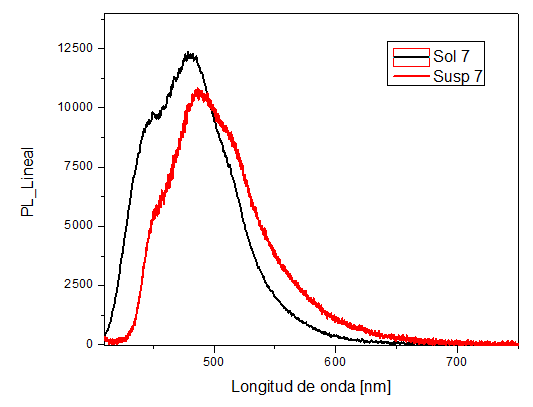
\includegraphics[width=0.65\textwidth]{resultados/sechgo/m7}
\end{subfigure}
\caption{Espectros de emisi\'on lineal de las muestras 6, 10 y 13 en soluci\'on y de las muestras 3 y 7 en soluci\'on y suspensi\'on de nanopart\'iculas.}
\label{emilinhgo}
\end{figure}

\begin{figure}[h]
\centering
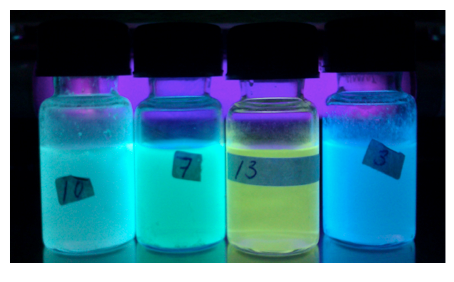
\includegraphics[width=0.45\textwidth]{resultados/sechgo/suspturbias}
\caption{De izquierda a derecha, fluorescencia de las muestras 10, 7, 13 y 3 en suspensi\'on bajo una l\'ampara UV como fuente de excitaci\'on.}\label{susphgo}
\end{figure}


La \'ultima columna de la tabla \ref{tablahgo} hace referencia al valor de $\Phi_f$ promedio tomando en cuenta un factor de correcci\'on\footnote{Este factor de correcci\'on se obtiene de las curvas de respuesta del PMT contenidas el manual de dicho equipo} proveniente de la sensibilidad de respuesta que el PMT tiene para distintas longitudes de onda. Es decir,  cuando la fluorescencia de la muestra de inter\'es y de la referencia (Rodamina 6G) tienen longitudes de onda similares, el PMT responder\'a de la misma manera en ambas muestras; sin embargo, si la muestra y la referencia emiten a diferentes longitudes de onda, es necesario introducir un factor de correci\'on.



\begin{table}[h]
\centering
\scalebox{0.82}{
\begin{tabular}{| l | c | c | c | c | c | r | }  %p{6.5cm} | c |
\hline
Muestra          & $\Phi_{f1}$ &$\Phi_{f2}$& $\Phi_{f Promedio}$&$\Phi_{fPromedio}$ /correcci\'on PMT  \\ \hline   %\multicolumn{8}{|c|}
Sol 3 	& 0.154	& 0.141	&0.148 & 0.09 \\ \hline
Sol 6         & 0.120     & 0.105	& 0.113 & 0.07    \\ \hline
Sol 7         & 0.430     & 0.236	& 0.333 & 0.20    \\ \hline
Sol 10 	& 0.266	& 0.255	&0.260 & 0.16 \\ \hline
Sol 13 	& 0.237	& 0.297	&0.267 & 0.27   \\ \hline
Susp 3 	& 0.279	& 0.148	&0.213 & 0.13    \\ \hline
Susp 7      &0.357     & 0.311      &0.335& 0.22  \\ \hline
\end{tabular} } 
\caption{ Valores obtenidos de eficiencia cu\'antica de fluorescencia $\Phi_f$ de las soluciones 3, 6, 7, 10 y 13 y las suspensiones 3 y 7.\label{tablahgo}}
\end{table}

Posteriormente se realizaron mediciones de $\sigma^{TPA}$ en un rango de 750 a 810 $nm$, para determinar \'este par\'ametro mediante la t\'ecnica de TPEF se utiliz\'o la ecuaci\'on \ref{finalsigma}, sin embargo, como los espectros de emisi\'on no lineal de la muestra de inter\'es y de referencia se adquirieron bajo las mismas condiciones, utilizando el mismo sistema de detecci\'on, entonces la eficiencia de colecci\'on de fluorescencia es la misma y $\eta_{ref}=\eta$; de igual manera, la potencia incidente fue la misma para todas las muestras $\langle P(t)\rangle_{ref}=\langle P(t)\rangle$. Asumiendo que $n_{ref}/n\approx 1$, el par\'ametro a calcular para conocer $\sigma^{TPA}$ es el valor de la integral del espectro de emisi\'on no lineal de la referencia y de la muestra de inter\'es $\langle F(t)\rangle_{ref}$ y $\langle F(t)\rangle$.

Las soluciones 3, 6, 13 y la suspensi\'on 3 no presentaron fluorescencia inducida por absorci\'on de dos fotones en el rango mencionado con anterioridad; sin embargo, los espectros de emisi\'on no lineal de las soluciones 7, 10, 13 y la suspensi\'on 7 se detectaron a todas las longitudes de onda de excitaci\'on. En la figura \ref{eminlhgo} se muestran los espectros adquiridos con una longitud de onda de excitaci\'on de 750 $nm$. 

\begin{figure}[h]
\centering
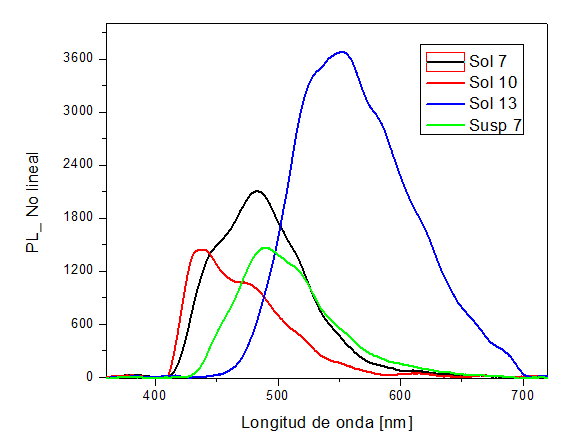
\includegraphics[width=0.85\textwidth]{resultados/sechgo/eminolinhgo}
\caption{Espectros de emisi\'on no lineal de las mol\'eculas 10 y 13 en soluci\'on y 7 en soluci\'on y suspensi\'on (Excitaci\'on a 750 $nm$).}\label{eminlhgo}
\end{figure}

Los valores obtenidos de secci\'on transversal de absorci\'on de dos fotones se muestran graficados en la figura \ref{tpahgo}. La soluci\'on 13 present\'o los valores m\'as altos de $\sigma^{TPA}$ en todas las longitudes de onda de excitaci\'on (menores a 600 $GM$) y el resto de las muestras presentaron valores menores de 300 $GM$. De los materiales org\'anicos con los que se trabajaron en este proyecto, este conjunto de mol\'eculas present\'o algunos de los valores m\'as bajos de eficiencias cu\'anticas de fluorescencia y $\sigma^{TPA}$, adem\'as la mayor\'ia de suspensiones acuosas de nanopart\'iculas se precipitaban inmediatamente despu\'es de ser fabricadas, volviendo las suspensiones m\'as turbias e inestables. Por ello no fue de inter\'es continuar con los estudios de absorci\'on no lineal y utilizar estos materiales como posibles marcadores celulares.



\begin{figure}[H]
\centering
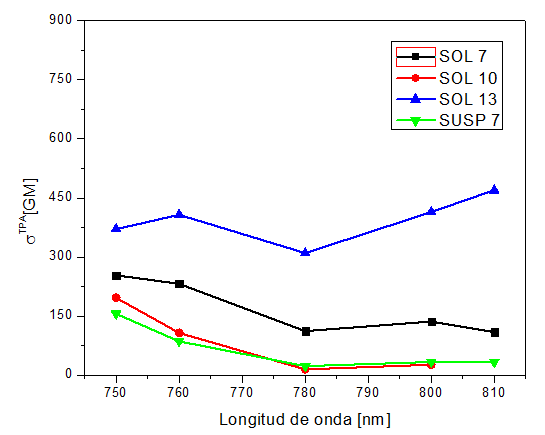
\includegraphics[width=0.85\textwidth]{resultados/sechgo/TPAhgo}
\caption{Epectros de absorci\'on no lineal de las mol\'eculas 10 y 13 en soluci\'on y 7 en soluci\'on y suspensi\'on}\label{tpahgo}
\end{figure}





%. En la figura \ref{X} se muestran los espectros de absorci\'on lineal molar $\epsilon$ de estas soluciones y suspensiones. La mayor absorci\'on se presenta en 
%. En la figura \ref{X} se muestran los espectros de absorci\'on lineal molar $\epsilon$ de estas soluciones y suspensiones. La mayor absorci\'on se presenta en 
%. En la figura \ref{X} se muestran los espectros de absorci\'on lineal molar $\epsilon$ de estas soluciones y suspensiones. La mayor absorci\'on se presenta en 
%. En la figura \ref{X} se muestran los espectros de absorci\'on lineal molar $\epsilon$ de estas soluciones y suspensiones. La mayor absorci\'on se presenta en 
%. En la figura \ref{X} se muestran los espectros de absorci\'on lineal molar $\epsilon$ de estas soluciones y suspensiones. La mayor absorci\'on se presenta en 

\section{Copol\'imero PF2/6-b-P3TMAHT}

Para este copol\'imero, cuya estructura qu\'imica se muestra en la figura \ref{copolimerito}, se realizaron dos soluciones y una suspensi\'on acuosa de nanopart\'iculas bajo condiciones distintas al resto de los materiales del proyecto. Era de inter\'es para este trabajo estudiar las propiedades \'opticas del copol\'imero anfif\'ilico en soluci\'on, utilizando como disolvente una mezcla de agua y THF (el material no es soluble en THF). 

En las dos soluciones realizadas se disolvi\'o el material en un volumen de agua- THF en proporci\'on 1:1 a concentraciones de $9.25 \times 10 ^{-6} M$ y $6.66\times 10^{-8} M$; para elaborar la suspensi\'on, a una concentraci\'on de $6.66\times 10^{-8} M$, se utiliz\'o dodecilsulfato s\'odico (SDS) como surfactante. Se manejaron bajas concentraciones para formar nanoagregados vesiculares y evitar las estructuras de tipo lamelar\cite{scherf}.

En la figura \ref{abscopo} se observan los espectros de absorci\'on molar del copol\'imero en soluciones y en suspensi\'on acuosa. En \'estos se aprecian dos m\'aximos alrededor de 370 y 450 $nm$ correspondientes a los dos bloques o dos distintos mon\'omeros polimerizados que constituyen este copol\'imero.

\begin{figure}[h]
\centering
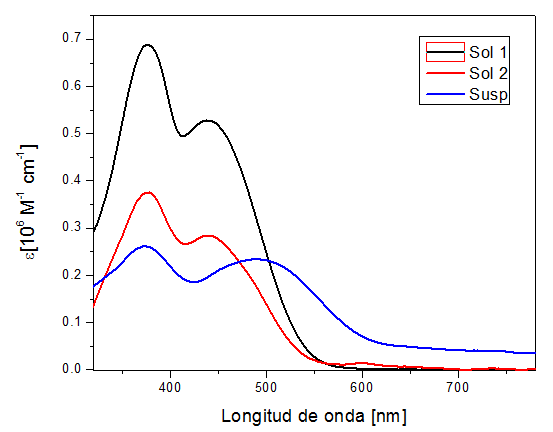
\includegraphics[width=0.85\textwidth]{resultados/copolimero/absmol}
\caption{Espectros de absorci\'on molar de soluciones y suspensi\'on. Concentraciones: \emph{Sol 1}- $9.25 \times 10 ^{-6} M$, \emph{Sol 2}- $6.66\times 10^{-8} M$ y \emph{Susp}- $6.66\times 10^{-8} M$.}\label{abscopo}
\end{figure}

La diferencia entre los espectros de las soluciones 1 y 2 (\emph{Sol 1} y \emph{Sol 2}) radica primordialmente en la intensidad de absorci\'on (Ver Figura \ref{absnormalizadita}), lo cual indica que a ambas concentraciones se forman el mismo tipo de estructuras vesiculares; adem\'as no presentaron esparcimiento. El espectro de la suspensi\'on present\'o una disminuci\'on de la absorci\'on, adem\'as del esparcimiento y un ensanchamiento y corrimiento hacia el rojo del m\'aximo que estaba alrededor de 450 $nm$ (\'unicamente un bloque), esto probablemente se debi\'o a la creciente algomeraci\'on que sufri\'o dicho bloque en el SDS.
 
\begin{figure}[h]
\centering
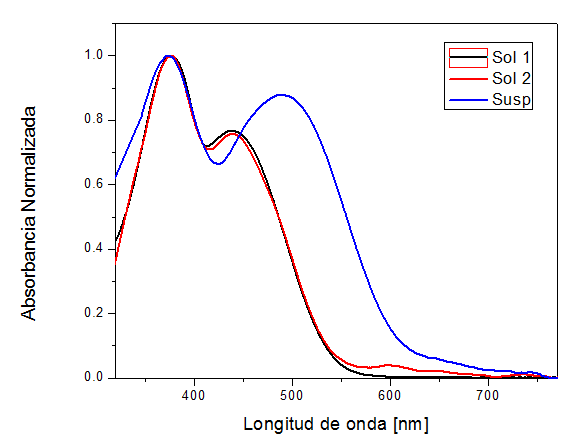
\includegraphics[width=0.65\textwidth]{resultados/copolimero/abs_norm}
\caption{Espectros de absorci\'on molar normalizados para la soluci\'on 1, 2 y una suspensi\'on acuosa.}\label{absnormalizadita}
\end{figure}

Posteriormente se adquirieron los espectros de emisi\'on lineal utilizando un diodo l\'aser como fuente de excitaci\'on, emitiendo a 370 $nm$. La emisi\'on de la suspensi\'on fue muy d\'ebil y no pudo detectarse; en la figura \ref{copoemilineal} se muestran los espectros de emisi\'on de las soluciones a concentraciones de $9.25 \times 10 ^{-6} M$ (\emph{Sol 1}) y $6.66\times 10^{-8} M$ (\emph{Sol 2}). La baja concentraci\'on de la soluci\'on 2 dificult\'o la detecci\'on de emisi\'on, como se muestra en la figura \ref{emilinnorm}, en donde se puede apreciar el ruido o luz de fondo. 

\begin{figure}[H]
\centering
\begin{subfigure}{0.49\textwidth}
\centering
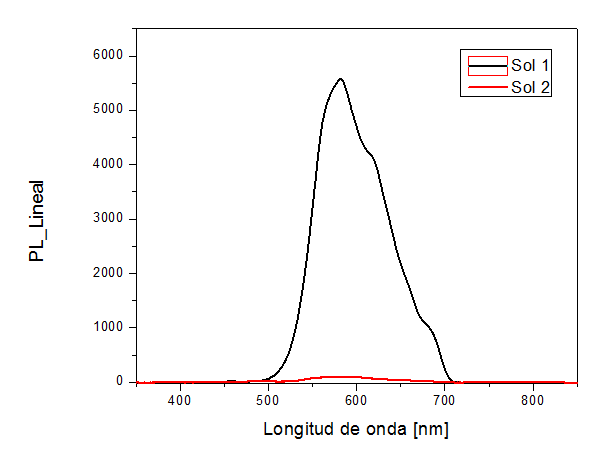
\includegraphics[width=\textwidth]{resultados/copolimero/pl_lineal}\caption{Emisi\'on lineal}\label{}
\end{subfigure}
\begin{subfigure}{0.47\textwidth}
\centering
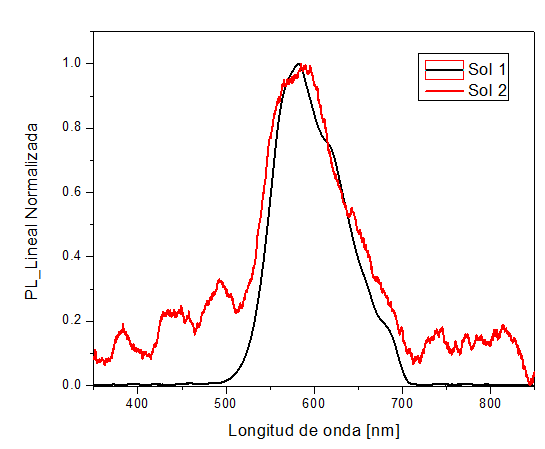
\includegraphics[width=\textwidth]{resultados/copolimero/pl_lineal_norm}\caption{Emisi\'on lineal normalizada}\label{emilinnorm}
\end{subfigure}
\caption{Espectros de emisi\'on lineal del copol\'imero en soluci\'on. Concentraciones: \emph{Sol 1}- $9.25 \times 10 ^{-6} M$ y \emph{Sol 2}- $6.66\times 10^{-8} M$ .}\label{copoemilineal}
\end{figure}

El valor de la eficiencia cu\'antica de fluorescencia ya era conocido, se reporta en la referencia \cite{scherf} y es $\Phi_f=0.16$. Tomando en cuenta lo anterior, finalmente se obtuvieron los espectros de emisi\'on no lineal para determinar la secci\'on transversal de absorci\'on de dos fotones en un rango de excitaci\'on de 760 a 810 $nm$. \'Unicamente se detect\'o la emisi\'on no lineal de la soluci\'on 1 a una concentraci\'on de $9.25 \times 10 ^{-6} M$; en la figura \ref{nolinealejemplos} se muestran algunos espectros de emisi\'on utilizando longitudes de onda de excitaci\'on de 760, 790 y 810 $nm$. Los valores obtenidos de $\sigma ^{TPA}$ de 760 a 810 $nm$ se muestran en la figura \ref{sigmacopo}. 



\begin{figure}[h]
\centering
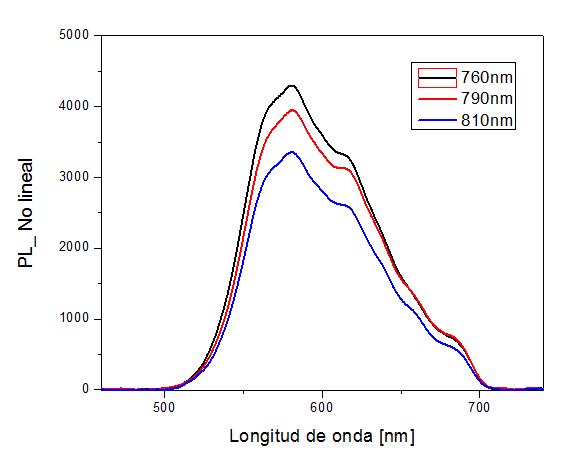
\includegraphics[width=0.69\textwidth]{resultados/copolimero/eminolineal}
\caption{Espectros de emisi\'on no lineal del copol\'imero en soluci\'on. Longitudes de excitaci\'on: 760, 790 y 810 $nm$.}\label{nolinealejemplos}
\end{figure}



\begin{figure}[H]
\centering
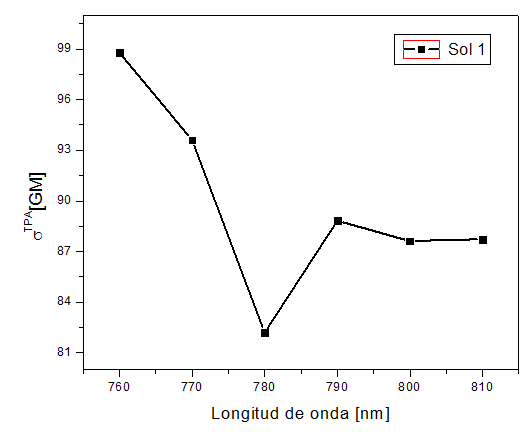
\includegraphics[width=0.68\textwidth]{resultados/copolimero/tpacopo}
\caption{Espectros de absorci\'on no lineal del copol\'imero en soluci\'on, c=$9.25 \times 10 ^{-6} M$.}\label{sigmacopo}
\end{figure}

Como se aprecia en la figura \ref{sigmacopo} hay un valor m\'inimo de $\sigma ^{TPA}$ en 780 $nm$; \'esto probablemente indique la separaci\'on entre los m\'aximos de absorci\'on de los dos bloques. Los valores de secci\'on transversal de absorci\'on de dos fotones para \'este copol\'imero en soluci\'on son muy bajos comparados con la literatura ($10^5 GM$) y con otros materiales estudiados en este trabajo; por ello no se estudi\'o la emisi\'on inducida por absorci\'on de dos fotones en otro rango de excitaci\'on. 
 
 
 


%%%%%%%%%%%%%%%%%%%%%%%%%%%%%%%%%%%%%%%%%%%%%%%%%%%%%%%%%%%%%%%%%%%%%%%%%%%
%%%%%%%%%%%%%%%%%%%%%%%%%%%%%%%%%%%%%%%%%%%%%%%%%%%%%%%%%%%%%%%%%%%%%%%%%%%
%%%%%%%%%%%%%%%%%%%%%%%%%%%%%%%%%%%%%%%%%%%%%%%%%%%%%%%%%%%%%%%%%%%%%%%%%%%
%%%%%%%%%%%%%%%%%%%%%%%%%%%%%%%%%%%%%%%%%%%%%%%%%%%%%%%%%%%%%%%%%%%%%%%%%%%
\section{Comparaci\'on de propiedades \'opticas entre sistemas moleculares dipolar, cuadrupolar y octopolar}

Inicialmente se prepararon soluciones en THF y suspensiones acuosas de nanopart\'iculas para las mol\'eculas 1NDS, 2NQS y 3NOS (Ver Figura \ref{ar2}) a una concentraci\'on de $6.25 \times 10^{-6} M$ utilizando CTAB. En la figura \ref{X} se muestran los espectros de absorci\'on lineal molar $\epsilon$ de estas soluciones y suspensiones. La mayor absorci\'on se presenta en el sistema octopolar, luego en el sistema cuadrupolar y finalmente en el sistema dipolar. 

\begin{figure}[h]
\centering
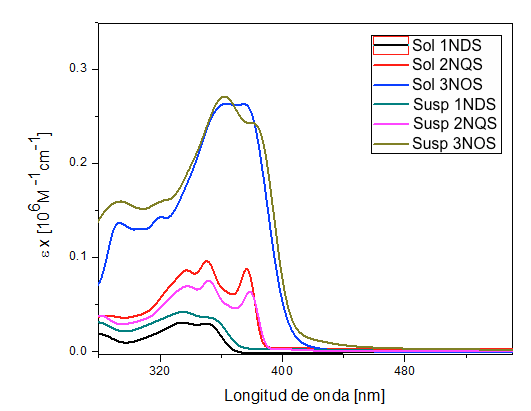
\includegraphics[width=0.85\textwidth]{resultados/sec1/comp}
\caption{Espectros de absorci\'on molar de 1NDS, 2NQS, 3NOS. Las etiquetas \emph{sol} y \emph{susp} se refieren a los sistemas moleculares en soluci\'on y suspensi\'on respectivamente}\label{X}
\end{figure}

Posteriormente se adquirieron los espectros de emisi\'on lineal de las soluciones y suspensiones a la misma concentraci\'on, utilizando un diodo l\'aser de 370 $nm$. Estos espectros se muestran en la figura \ref{los3espemilineal} y se puede apreciar que la mayor emisi\'on se presenta en el sistema octopolar en soluci\'on y en suspensi\'on de nanopart\'iculas. En todos los sistemas moleculares la emisi\'on del material en soluci\'on fue mayor que en suspensi\'on de nanopart\'iculas y en el caso del sistema octopolar 3NOS, el espectro de emisi\'on en suspensi\'on sufri\'o un corrimiento hacia el rojo comparado con el espectro en soluci\'on (Ver Figura \ref{3nsolsusp}); esto se atribuye las interacciones moleculares ocasionadas por el confinamiento del material al formar las nanopart\'iculas.  



\begin{figure}
\centering
\begin{subfigure}{\textwidth}
\centering
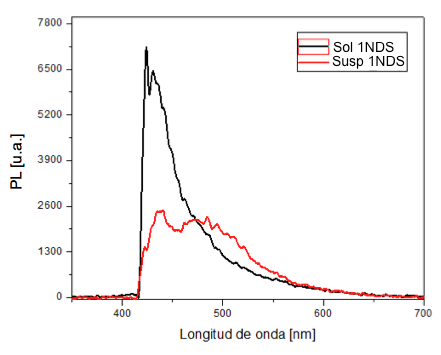
\includegraphics[width=0.65\textwidth]{resultados/sec1/1n}
\end{subfigure}
\begin{subfigure}{\textwidth}
\centering
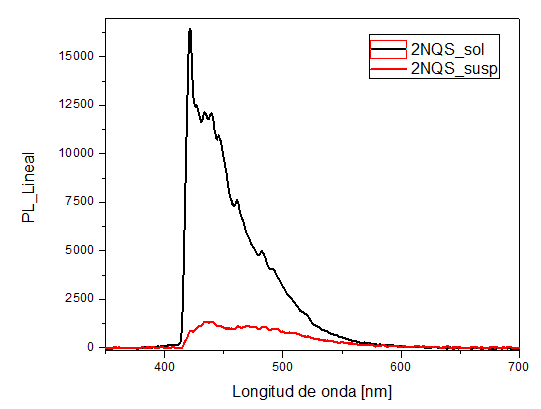
\includegraphics[width=0.65\textwidth]{resultados/sec1/2n}
\end{subfigure}
\begin{subfigure}{\textwidth}
\centering
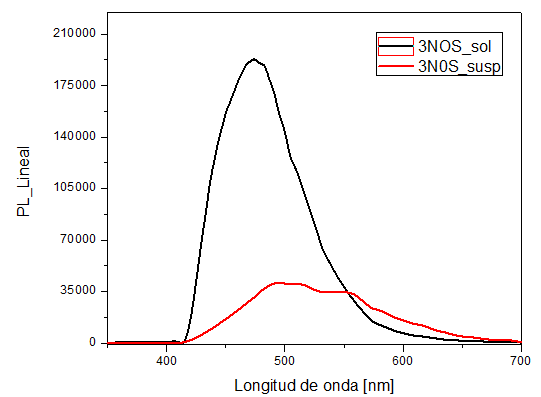
\includegraphics[width=0.65\textwidth]{resultados/sec1/3n}
\end{subfigure}
\caption{Espectros de emisi\'on lineal de 1NDS, 2NQS y 3NOS en soluci\'on y suspensi\'on de nanopart\'iculas}
\label{los3espemilineal}
\end{figure}



\begin{figure}[h]
\centering
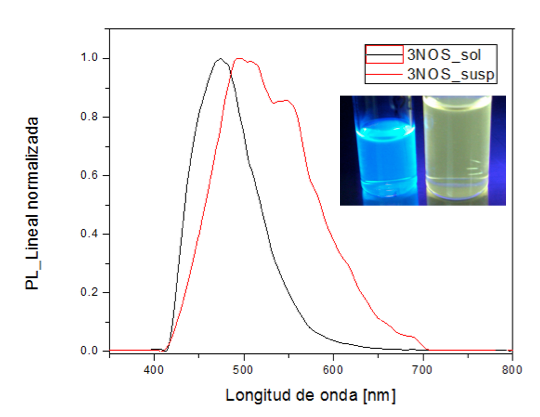
\includegraphics[width=0.85\textwidth]{resultados/sec1/emilinealnorm3N}
\caption{Espectros normalizados y fluorescencia visible de 3NOS en soluci\'on (azul) y suspensi\'on (amarilla)}\label{3nsolsusp}
\end{figure}


En comparaci\'on con el sistema octopolar, la emisi\'on lineal (y no lineal como se ver\'a en seguida) de los sistemas dipolar y cuadrupolar fue muy d\'ebil. Por ello \'unicamente fue de inter\'es medir varias veces la eficiencia cu\'antica de fluorescencia del sistema octopolar 3NOS, en soluci\'on y suspensi\'on acuosa de nanopart\'iculas utilizando CTAB y nuevamente a una concentraci\'on de $6.25 \times 10^{-6} M$; los valores obtenidos utilizando la ecuaci\'on \ref{final} y un factor de correci\'on de 0.6 para la soluci\'on octopolar (por la respuesta del PMT) se muestran en la tabla \ref{tablita}. 

\begin{table}[H]
\centering
\scalebox{0.82}{
\begin{tabular}{| l | c | c | c | c | c | c | c | c | r | }  %p{6.5cm} | c |
\hline
 3NOS           & $\Phi_{f1}$	&$\Phi_{f2}$ &$\Phi_{f3}$&$\Phi_{f4}$&$\Phi_{f5}$& $\Phi_{fPromedio}$&$\Phi_{fPromedio}$ /correcci\'on PMT  \\ \hline   %\multicolumn{8}{|c|}
Soluci\'on &    0.457&	0.539& 0.341	& -	& -	&0.44& 0.26 \\ \hline
Suspensi\'on & 	0.129 &	 0.191& 0.094 & 0.225& 0.226	& 0.17&0.17 \\ \hline
\end{tabular} } 
\caption{ Valores obtenidos de eficiencia cu\'antica de fluorescencia $\Phi$ para el sistema octopolar  \label{tablita}}
\end{table}


Las mediciones de $\sigma^{TPA}$ en el rango de 740 $nm$ a 840 $nm$ para los tres sistemas moleculares se realizaron a una concentraci\'on de $6.25\times 10^{-6} M$. A esta concentraci\'on los espectros de emisi\'on no lineal de los sistemas dipolar y cuadrupolar tanto en soluci\'on como en suspensi\'on estuvieron por debajo del nivel de detecci\'on del arreglo experimental (Ver Figura \ref{nel}); sin embargo, los espectros del sistema octopolar para algunas longitudes de onda de excitaci\'on se muestran en la figura \ref{sip} y los valores de $\sigma^{TPA}$ se presentan en la gr\'afica de la figura \ref{tpaprimeros}.

\begin{figure}
\centering
\begin{subfigure}{\textwidth}
\centering
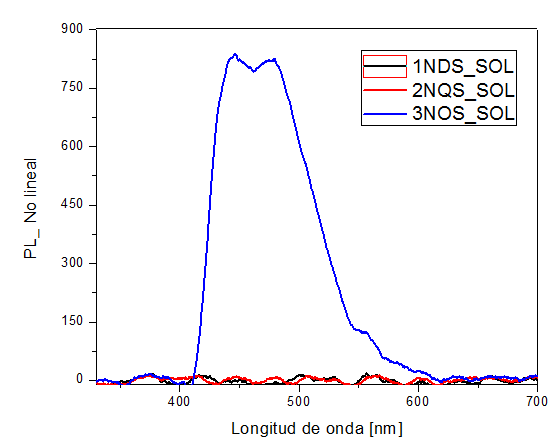
\includegraphics[width=0.6\textwidth]{resultados/sec1/nojalo}
\caption{Espectros de emisi\'on no lineal para 1NDS, 2NQS y 3NOS en soluci\'on con un haz de excitaci\'on a 760 $nm$ }\label{nel}
\end{subfigure}
\begin{subfigure}{\textwidth}
\centering
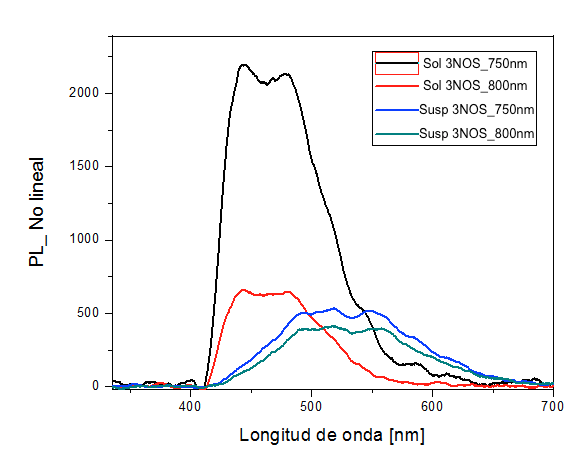
\includegraphics[width=0.7\textwidth]{resultados/sec1/sijalo}
\caption{Comparaci\'on de espectros de emisi\'on no lineal para 3NOS en soluci\'on y suspensi\'on para diferentes longitudes de onda de excitaci\'on }\label{sip}
\end{subfigure}
\caption{Espectros de emisi\'on no lineal}
\label{ghghh}
\end{figure}

\begin{figure}[h]
\centering
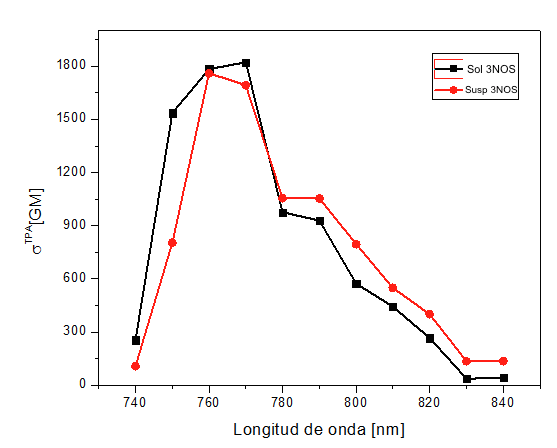
\includegraphics[width=0.7\textwidth]{resultados/sec1/TPA_1}
\caption{Espectro de absorci\'on no lineal de 3NOS en soluci\'on y suspensi\'on}\label{tpaprimeros}
\end{figure}

Posteriormente se realizaron pruebas para recubrir las nanopart\'iculas de la mol\'ecula octopolar con PEG 5000 sin utilizar surfactantes. Se prepar\'o una suspensi\'on acuosa de nanopart\'iculas a una concentraci\'on de $6.43 \times 10^{-6}M$, utilizando una concentraci\'on de PEG 5000 de $5\times 10^{-6} M$. En la figura \ref{grr} se muestra una comparaci\'on de los espectros de absorci\'on (\ref{abspeg1}) y emisi\'on lineal (\ref{emipeg1}) de la mol\'ecula octopolar en soluci\'on, suspensi\'on utilizando CTAB y suspensi\'on de nanopart\'iculas utilizando PEG 5000, todas a la misma concentraci\'on $6.43 \times 10^{-6}M$. 

\begin{figure}
\centering
\begin{subfigure}{0.5\textwidth}
\centering
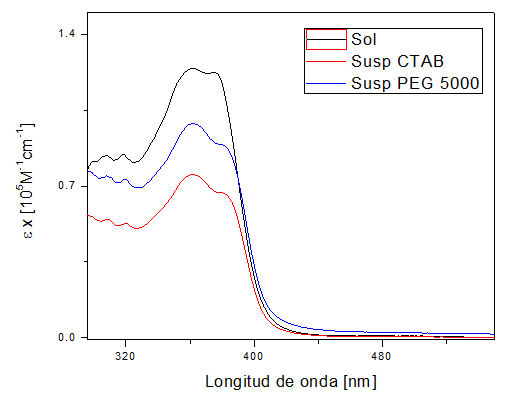
\includegraphics[width=\textwidth]{resultados/sec1/abs_peg5000}
\caption{Absorci\'on molar lineal }\label{abspeg1}
\end{subfigure}
\begin{subfigure}{0.49\textwidth}
\centering
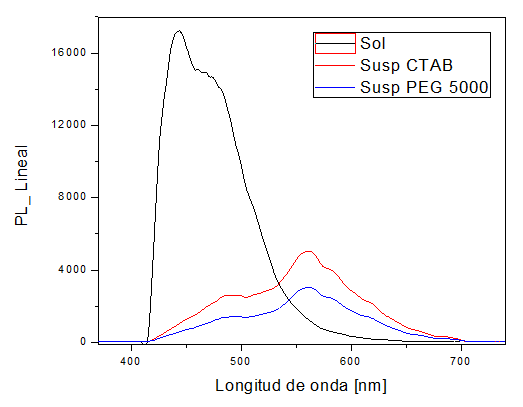
\includegraphics[width=\textwidth]{resultados/sec1/emi_peg5000}
\caption{Emisi\'on lineal }\label{emipeg1}
\end{subfigure}
\caption{Espectros de la mol\'ecula octopolar en soluci\'on \emph{Sol} y  en suspensiones con CTAB \emph{Susp CTAB} y PEG \emph{Susp PEG 5000}}
\label{grr}
\end{figure}

Se realizaron cinco mediciones de eficiencia cu\'antica de fluorescencia para la suspensi\'on acuosa de nanopart\'iculas funcionalizadas con PEG 5000 obteniendo una eficiencia promedio $\Phi_{f_{Promedio}}$ de 0.14. Tambi\'en se midi\'o la secci\'on transversal de absorci\'on de dos fotones de esta suspensi\'on para las siguientes longitudes de onda de excitaci\'on: 760, 780, 800 y 815 $nm$; los valores de $\sigma^{TPA}$ para la mol\'ecula octopolar en soluci\'on, suspensi\'on con CTAB y suspensi\'on con PEG 5000 se muestran en la gr\'afica de la figura \ref{valoressigmapeg1}.

\begin{figure}[h]
\centering
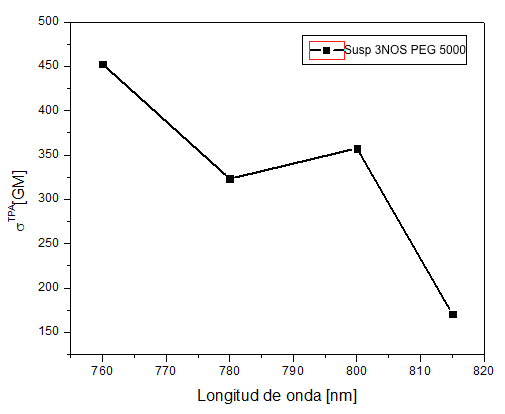
\includegraphics[width=0.7\textwidth]{resultados/sec1/TPA_PEG1}
\caption{Espectro de absorci\'on no lineal para 3NOS en soluci\'on \emph{Sol} y suspensiones con CTAB \emph{Susp CTAB} y PEG 5000, \emph{Susp PEG 5000}}\label{valoressigmapeg1}
\end{figure}

En este trabajo la mol\'ecula octopolar fue uno de los sistemas moleculares  de mayor inter\'es, por ello se determinaron los valores de $\sigma^{TPA}$ en el rango de longitudes de onda incidentes de 650 a 760 $nm$ implementando el arreglo \'optico de TPEF como se explic\'o en la secci\'on \ref{laserchidote}. En este rango se determin\'o $\sigma^{TPA}$ para la mol\'ecula 3NOS en soluci\'on a una concentraci\'on de $6.43 \times 10^{-6} M$; sin embargo, debido a la sensibilidad del arreglo y al nivel de detecci\'on, a ciertas longitudes de onda no pudo determinarse $\sigma^{TPA}$. Los resultados se muestran en la figura \ref{valoressigmafs} junto con los resultados obtenidos anteriormente para la soluci\'on en el primer rango, de 740 a 840 $nm$ (Ver Figura \ref{tpaprimeros}).

\begin{figure}[h]
\centering
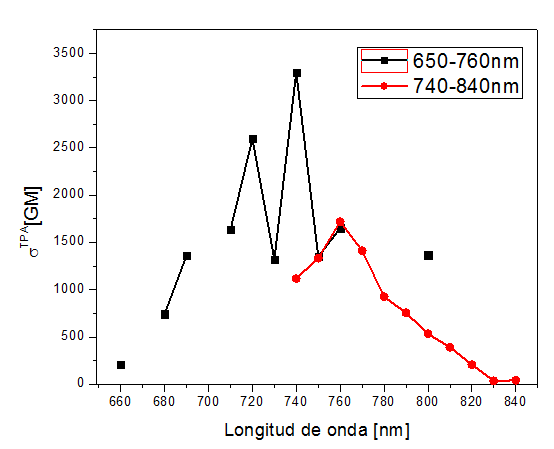
\includegraphics[width=0.7\textwidth]{resultados/sec1/TPA_femto}
\caption{Espectros de absorci\'on no lineal para 3NOS en soluci\'on de 650--760 nm y de $740-840nm$}\label{valoressigmafs}
\end{figure}

Posteriormente se realiz\'o una funcionalizaci\'on de nanopart\'iculas de la mol\'ecula octopolar, utilizando ahora el PEG 2000. Se prepar\'o una suspensi\'on acuosa de nanopart\'iculas sin CTAB a una concentraci\'on de $6.43 \times 10^{-6} M$ y con una concentraci\'on de PEG 2000 en la suspensi\'on de $6\times 10^{-4} M$. En la figura \ref{temi} se muestran un par de im\'agenes de esta suspensi\'on adquiridas con un microscopio electr\'onico de transmisi\'on o TEM por sus siglas en ingles, de la marca Philips modelo XL; los di\'ametros de las nanopart\'iculas van de 16.8 a 33.7 $nm$. 

\begin{figure}[h]
\centering
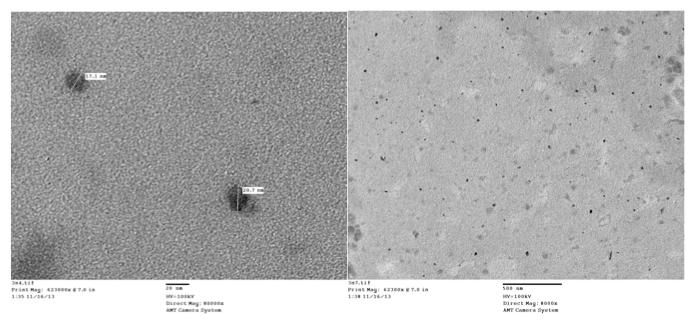
\includegraphics[width=\textwidth]{resultados/sec1/tem}
\caption{Im\'agenes TEM con escala de 20 y 500 $nm$}\label{temi}
\end{figure}

El PEG 2000 facilita la funcionalizaci\'on de nanopart\'iculas porque tiene m\'as grupos funcionales que el PEG 5000 como se mencion\'o en la secci\'on \ref{pegis}, adem\'as las suspensiones fabricadas con PEG 2000 fueron m\'as estables; en un tiempo de almacenamiento de m\'as de cinco meses a temperatura ambiente la suspensi\'on de nanopart\'iculas de 3NOS no se precipit\'o. Por ello y por las propiedades \'opticas que present\'o la mol\'ecula octopolar se decidi\'o internalizar esta suspensi\'on acuosa de nanopart\'iculas funcionalizadas con PEG 2000 en la l\'inea celular X.

Se internalizaron 500 $\mu l$ de la suspensi\'on a una concentraci\'on de $6.43 \times 10^{-6} M$ ...  


\section{Nanopart\'iculas del pol\'imero PMC300} 


\begin{figure}[H]
\centering
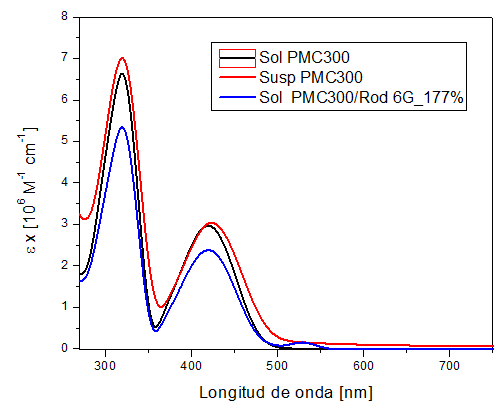
\includegraphics[width=0.85\textwidth]{resultados/pmc300/abs1}
\caption{Im\'agenes TEM con escala de 20 y 500 $nm$}\label{pmc_abs1}
\end{figure}
